\documentclass[a4paper,12pt]{article}
\usepackage{mathtools, amsmath, listings,graphicx, svg, csquotes}
\graphicspath{ {images/} }
\begin{document}
\lstset{language=Python}

\title{A Critique of Dominant Random Graph Models}

\author{Grady Ward}

\maketitle

\subsection*{Dominant Models of Random Graphs}

The two dominant models for `random', undirected graphs were both defined by Erdos and Reyni in TODO.
The first is a model which selects an adjacency matrix at random from the set of all square binary matrices.
The second constructs each edge with an independent and fixed probability. 
Both models have been studied at length, and they have been proven asymptotically alike. 
Though these models make intuitive sense, we ought examine why they have domainated the study of `random' graphs.

In the random matrix model it is clear to see that properties of `random' matrices can be applied to `random' graphs.
Additionally, we can use some existing proofs and proof techniques in integer theory to advance `random' graph theory by treating the matrix as a bitstring. 
This random graph generator has been useful because it links random matrix/integer theory to `random' graph theory.

In the independently random edge model, we can easily calculate many properties of the graph that are of interest to graph theoreticians.
For example, the probability distribution of the number of triangles in a graph is a simple summation of products.
Additionally, this model succinctly describes many 'real-world' problems that do not require much imagination to dream up.
This model of random graphs has been impactful because it allows graph theoreticians to concretely discuss many of the properties that they are interested in, and connects graph theory to its applications.

In short, both models have stuck precisely because they marry an intuitive model with the tools to easily discuss the properties that their `random' graphs have.

\subsection*{Disconnect from Algebra}

Neither model for `random' graph generation treats graphs as algebraic objects.
It was shown by TODO in TODO that the number of matrices which represent a graph \(G\) is
\[| Matrices(G) | = \frac{N!}{| Aut(G) |}\]
where \(Aut(G)\) is the automorphism group of \(G\).
As a consequence, in perfectly symmetric graphs (such as \(K_i\)), there is only one way to represent \(G\).
In contrast, most graphs only possess a trivial automorphism, and thus can be represented by \(N!\) distinct matrices.
Thus, in the proposed `random' generators, the odds of picking out one algebraic object can be a factor of \(N!\) larger than picking out another. 

This should make the reader question how `random' graph generators fit into our colloquial understanding of randomness.
Common understandings of 'random selection from a set' implies uniform probability of selecting elements.
In graph theory, labeling and representation are rarely factors that impact our calculations, thus our default mode of understanding is found in most papers: 'irrespective of isomorphisms'.
Thus, we ought question the validity of models which heavily bias for some graphs over others by ignoring isomorphism.
The focus of this article is the quantification of the disconnects between these `random' models, and random graphs as algebraic objects.

\subsection*{Strength of Erdos Renyi Distributional Assumption}

The number of graphs (\(N_{Graphs}\))of a given size is still not available as a closed form, but has been computed to 19 vertices (OEIS A000088) (Column (1)).
The number of valid binary matrices that represent undirected non-looped graphs is trivially expressed as \(N_{Matrices} = 2^{.5(N^2 - N)}\) (Column (2)).
Dividing these sequences gives us the average number of matrix representations for graphs of size \(N\) (Column (3)).
Clearly, this average must fall between 1 and the maximum number of representations, which is simply \(N!\).
If we divide the average by the maximum, we see that it asymptotically is climbing to 1 (Column (4), Figure 1).

This means that `random' graph generators are closer to an algebraic concept of random as the size of the graph increases, 
as the average graph grows to asymptotically be equivalent in number of representations to the maximum.

\begin{tabular}{ r | r | r || r ||| r}
  \(N\) & (1) \(N_{Graphs}\) & (2) \(N_{Matrices}\) & (3) \(Avg(Mats(G))\) & (4) = (3) / \(N!\) \\
  \hline			
  0 & \(1\) & \(1\) & \(1.000\) & 1.00000 \\
  1 & \(1\) & \(1\) & \(1.000\) & 1.00000 \\
  2 & \(2\) & \(2\) & \(1.000\) & 0.50000 \\
  3 & \(4\) & \(8\) & \(2.000\) & 0.33333 \\
  4 & \(11\) & \(64\) & \(5.800\) & 0.24242 \\
  5 & \(34\) & \(1028\) & \(30.12\) & 0.25098 \\
  6 & \(156\) & \(3.2 * 10^4\) & \(210.0\) & 0.29174 \\
  7 & \(1044\) & \(2.1 * 10^6\) & \(2009\) & 0.39856 \\
  8 & \(1.2 * 10^{4}\) & \(2.7 * 10^{8}\) & \(2.2 * 10^{3}\) & 0.53925 \\
  9 & \(2.7 * 10^{5}\) & \(6.9 * 10^{10}\) & \(2.5 * 10^{5}\) & 0.68946 \\
  10 & \(1.2 * 10^{7}\) & \(3.5 * 10^{13}\) & \(2.9 * 10^{6}\) & 0.80764 \\
  11 & \(1.0 * 10^{9}\) & \(3.6 * 10^{16}\) & \(3.5 * 10^{7}\) & 0.88577 \\
  12 & \(1.7 * 10^{11}\) & \(7.4 * 10^{19}\) & \(4.5 * 10^{8}\) & 0.93308 \\
  13 & \(5.1 * 10^{13}\) & \(3.0 * 10^{23}\) & \(6.0 * 10^{9}\) & 0.96106 \\
  14 & \(2.9 * 10^{16}\) & \(2.5 * 10^{27}\) & \(8.5 * 10^{10}\) & 0.97749 \\
  15 & \(3.1 *10^{19}\) & \(4.0 * 10^{31}\) & \(1.3 * 10^{12}\) & 0.98708 \\
  16 & \(6.4 * 10^{22}\) & \(1.3 * 10^{36}\) & \(2.1 * 10^{13}\) & 0.99264 \\
  17 & \(2.5 * 10^{26}\) & \(8.7 * 10^{40}\) & \(3.5 * 10^{14}\) & 0.99584 \\
  18 & \(1.8 * 10^{30}\) & \(1.1 * 10^{46}\) & \(6.4 * 10^{15}\) & 0.99766 \\
  19 & \(2.5 * 10^{34}\) & \(3.0 * 10^{51}\) & \(1.2 * 10^{17}\) & 0.99869 \\
  \hline  
\end{tabular}

\begin{figure}[htbp]
  \centering
  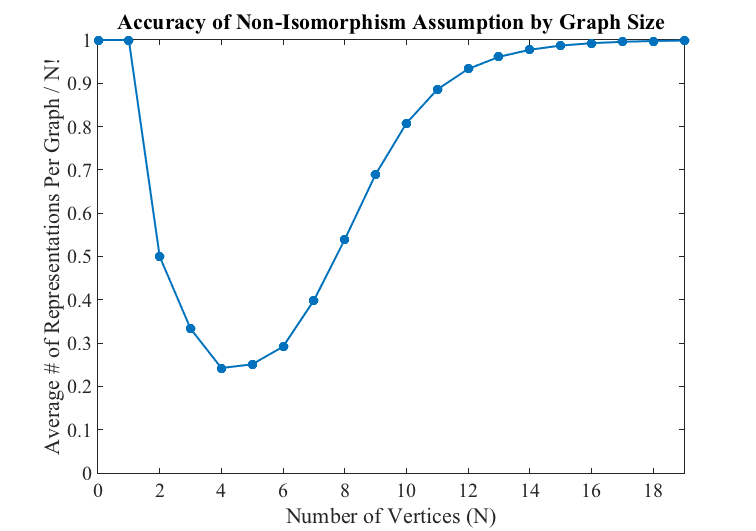
\includegraphics[scale=.45]{accuracy-of-assumption}
\end{figure}

\subsection*{Analysis}

We can explicitly state the assumption of the Erdos-Reyni random graph models as follows:
\begin{displayquote}
The models assume that the number of matrix representations of any two given graphs is asymptotically equal.
\end{displayquote}

We describe the representation distribution for \(N\) (\(RD_N\)) as the distribution of the number of ways to representing each graph of size \(N\) as a matrix.
This assumption is concerned with the \emph{variance} of this distribution, which it claims approaches zero.

The work that we have done in this article centers around the mean of this distribution, but basic statistical analysis can transform this information about means into information about the variance of the distribution. We will conclude two things from some simple statistical analysis:
\begin{itemize}
	\item{Asymptotically, this assumption holds for large values of \(N\)}
	\item{For small values of \(N\), this assumption is not only wrong, but leads to poorly selected distributions}
\end{itemize}

To prove the first, consider that the range of \(RD_N\) is \([1, N!]\). 
If (as we have for large N), the mean is close to N!, we know that the distribution is heavily skewed left.
We also know that \(RD_N\) is a discrete distribution with known possible values.
Since every value must be of the form \(\frac{N!}{K}\) where \(K\) is an integer, we know that if any value in the distribution is confirmed to be above \(.5 * N!\), then it equals \(N!\). 
Since we know that the distribution has a large proportion of its values at \(N!\), we will describe the proportion of values at that value as \(Prop_{Top}\).

In order to create a lower bound for what \(Prop_{Top}\) could be, we will make an imperfect assumption. 
Though flawed, it can \emph{only increase the variance of the distribution}.
We will assume that the other piece of the distribution is located at zero. 
We use this simplifying assumption to solve for the minimum \(Prop_{Top}\) possible given an average number of representations as in column (3).
\[ Prop_{Top} * N! + (1 - Prop_{Top}) * 0 \geq MeanReps_{(3)}\] 
\[ Prop_{Top} \geq MeanReps_{(4)} \]

If we now use the equation for variance of a discrete random variable, we can quickly find how the variance of the \(RD_N\) trends to zero:

\[Var(RD_N) = \sum_{i=0}^P p_i (x_i - \mu)^2 \leq (1 - P_T) (\mu - 0)^2 + (P_T) (1 - \mu)^2\]
\[Var(RD_N) \leq \mu^2 - P_T \mu^2 + P_T - 2 P_T \mu + P_T \mu^2 = (P_T - \mu)^2\]

And by observation of the fact that \(P_T \geq \mu, P_T < 1,\) and \(\lim_{N \to \infty}\mu =  1\), we know that \(\lim_{N \to \infty} Var(RD_N) = 0\).

The second proof is much simpler: Just look at the distribution for a small value of \(N\).
We do a Chi-Squared goodness of fit test to see if there is a statistically significant difference between the distributions, and there is, for \(N <= 10\).

\subsection*{Conclusions}

In this article, we discussed why the established `random' graph generators are popular in the literature.
That popularity has overshadowed how the assumptions baked in to the models do not hold up for small values of \(N\).
We then introduced a metric which we can use as an analogue for the validity of the models at different levels of \(N\).
We then showed how the explicit assumption fundamental to the models can easily be proven to hold in asymptotic analysis.
However, we also showed how the model's assumptions fail at small values of \(N\).

Luckily, generating random graphs of small size is a task that we have the capability to solve perfectly (within an algebraic context).
One could easily set up a database of all of the graphs with less than 12 vertices, and pull randomly from it.

However, there are issues remaining with this analysis. 
It doesn't justify the metric of average number of matrices.
It also only quantifies the number of graphs for which Erdos Renyi Random Models are insufficient as a proportion of all matrices, not as a proportion of all graphs.
Even in this analysis (which attempts to reject this established vernacular) the convenience of matrix analysis is a powerful temptation.

\end{document}